\documentclass[../Dissertation.tex]{subfiles}

\begin{document}
\section{Evaluation of experimental design}
\textbf{\color{red}
\begin{itemize}
    \item clear result presentation
    \item explain problems and difficulties
    \item demonstrate understanding of results
    \item discuss further work
\end{itemize}
}
\emph{
\begin{itemize}
	\item Duration of training
	\item volume of data gathered
	\item (im)practicalities - power consumption? 
	\item limitations - single optimisation metric
	\item Criticism of methodology
	\item Distiller only supports a single kind of network thinning, so mixing channel and filter pruning was not possible at this time
\end{itemize}
}

\textbf{Challenges}
\begin{itemize}
    \item Very little activity on the distiller repository in the last 6 months
    \item Distiller bugs - distiller shadows the namespace of the standard library python parser module, the path distiller uses to resume a model that has been thinnified is broken - fixed in my fork
    \item 
\end{itemize}
The size of the pruned networks is not measured.



\section{Evaluation of results}
\emph{
\begin{itemize}
	\item Summary of results per model/dataset
	\item Deep dive into results, detailed visualisations of accuracy \& latency tradeoffs (maybe example with poor quality sensitivity analysis vs higher quality layer selection)
\end{itemize}
}

Section~\ref{sec}

\subsection{Experiment 1: Rapid pruning}\label{sec:FastPruningPhase}

\begin{figure}[H]
    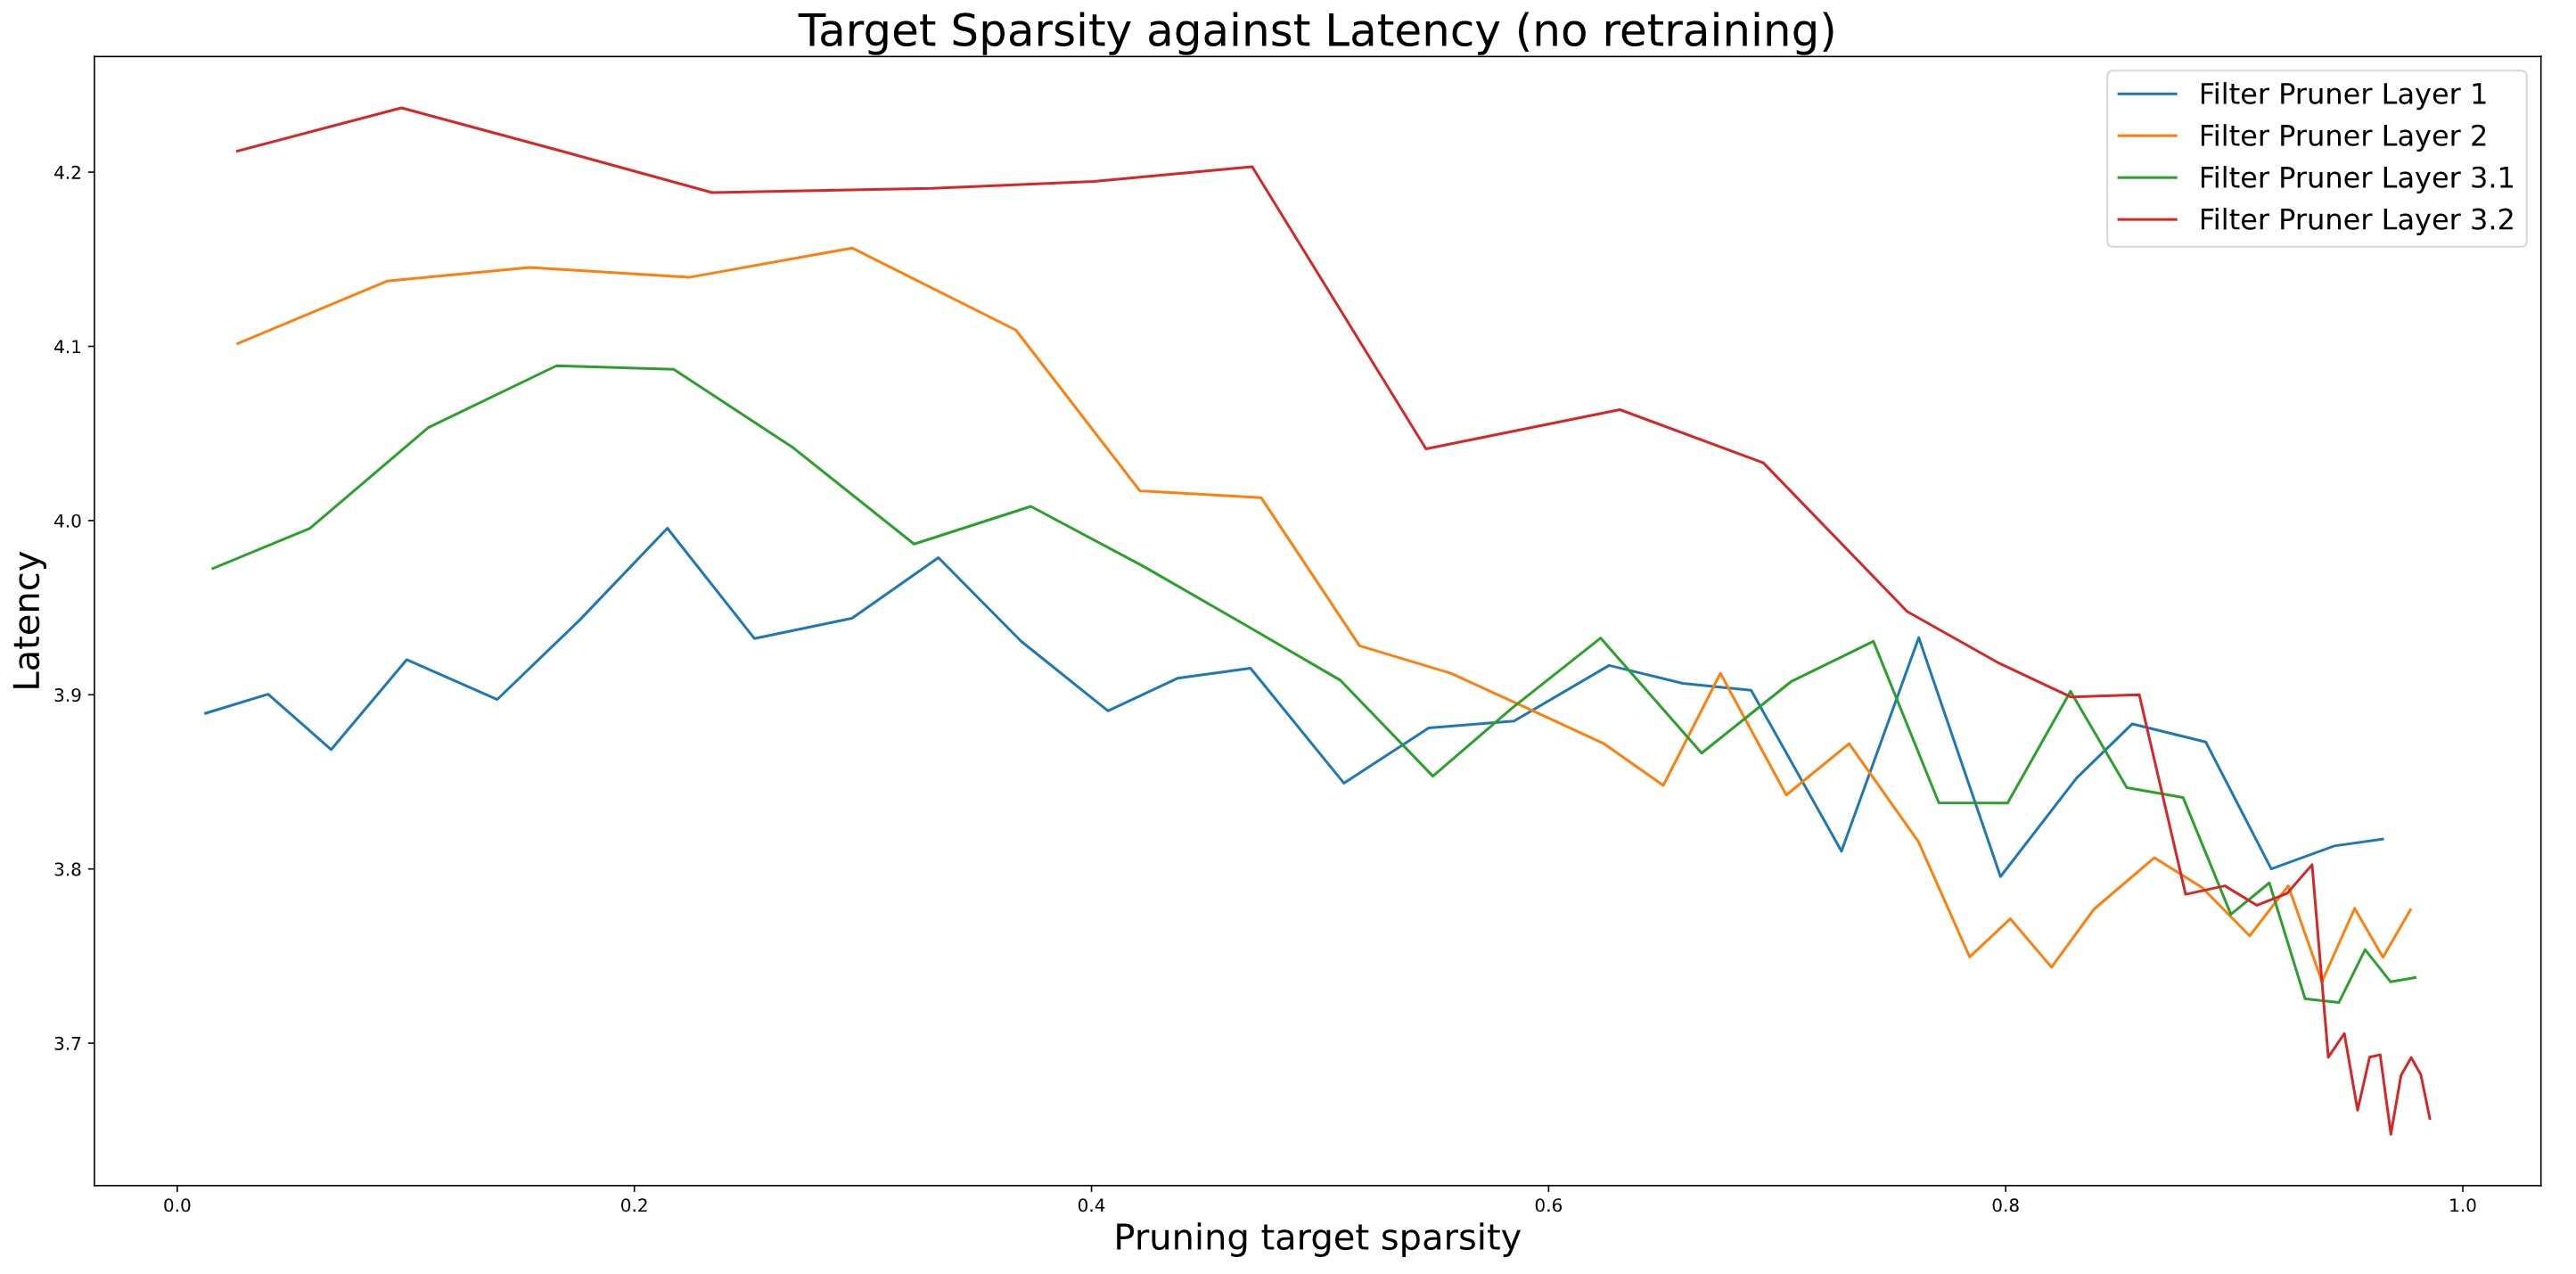
\includegraphics[width=1\textwidth]{TargetSparsityVsLatency_No_Retrain.jpg}
    \caption{Each pruner target sparisity plotted against mean Latency per bin.}
    \label{fig:fastPruneParamVSLatency}
\end{figure}

During this phase of the experiment we gathered data to observe how pruning would affect latency, this was useful as an initial proof of concept.
This phase of the experiment was very time efficient, we were able to perform 1631 runs with around 18 hours of compute time; each run usually lasted between 24-55 seconds. 
As discussed in section~\ref{sec:ex1} for this experiment we set the training epochs to 0 and set the target metric to minimize latency. 
Figure~\ref{fig:fastPruneParamVSLatency} shows the mean Latency computed by using equal width binning, where each bin represents parameter values inside each discretized 0.02 range between 0.0 and 1.0.
This chart does obfuscate any relationship between the parameters, however we can see how the filter pruner on Layer 3.2 (red) has a much greater impact on latency than the Pruner on Layer 1 (blue), this is also supported by computing the correlation between these values, see Table~\ref{tab:fastPruneCorrelations}, where `Filter Pruner Layer 3.2' has a strong negative correlation with Latency indicating that increasing the desired sparsity has a more dramatic effect on latency than `Filter Pruner Layer 1'.

\singlespacing
\begin{table}[H]
    \centering
    \begin{tabular}{@{}cp{26mm}p{26mm}p{26mm}p{26mm}@{}}
    \toprule
    \textbf{Metric}  & \textbf{Filter Pruner  Layer 1} & \textbf{Filter Pruner Layer 2} & \textbf{Filter Pruner Layer 3.1} & \textbf{Filter Pruner Layer 3.2} \\ \midrule
    \textbf{Latency} & $-0.11259$                        & $-0.552583$                      & $-0.40775$                         & $-0.80726$                         \\
    \textbf{Top1}    & $0.004462$                        & $-0.071923$                      & $-0.104505$                        & $-0.152767$                        \\ \bottomrule
    \end{tabular}
    \caption{Correlations between each target sparsity parameter and the metric being measured.}
    \label{tab:fastPruneCorrelations}
\end{table}
\doublespacing

We found that the degree to which we prune was not at all indicative of the resulting accruacy of the network before retraining, for example we observed networks with low desired sparsity accross the board that had a much lower Top1 accuracy, than networks that were pruned with much higher targets (See models~\ref{sec:golden-sweep-523}).
It is interesting to note how weakly the pruning targets correlate with Top1 accuracy, this indicates that the relationship between accuracy and pruning is more complex than the naive perception that pruning less has a smaller accuracy impact.
Observation of this weak correlation with Top1 prompted us to begin logging this initial set of metrics in addition to the metrics we logged as described in the Experimental Design Section~\ref{sec:metricsandparams}, we watched this data in the event that some pattern that might be indicative of how well a pruned network can recover accuracy before retraining has begun will emerge.

We were unfortunately unable to identify any such pattern from the data we gathered, due to the stochastic nature of pruning and retraining coupled with the fact that our methodology neccessitated changing the pruning parameters each run


\subsection{Experiment 2: Target Latency}

\subsection{Experiment 3: Target Top1}

\textbf{Interesting observations}
\begin{itemize}
    \item The models that lost all predictive power due to overpruning were not the fastest, even when targeting only latency.
    \item The relationship between more pruning and lower latency is not as simple as you get a faster model with fewer tensors
    \item When targeting accuracy we found models with as low latency when targeting latency directly.
    \item When targeting latency we found models with as high accuracy as when targeting accuracy directly.
    \item Surprising to see that retraining reduces the latency also
\end{itemize}

\end{document}